\documentclass[11pt]{article}
\usepackage{fancyhdr}
\usepackage[letterpaper, margin=1in]{geometry}
%\usepackage{indentfirst}
\usepackage{graphicx}
\usepackage{amsmath}
\usepackage{amssymb}
\usepackage{siunitx}
\sisetup{detect-weight=true, detect-family=true} % makes siunitx follow font formatting like bold, italic, etc.
\usepackage{cancel}
\usepackage{isotope}
\usepackage{listings}
\usepackage[dvipsnames,table]{xcolor}
\usepackage{xspace}
\usepackage{booktabs} % makes tables pretty
\usepackage{longtable} % for long tables
\usepackage{multirow} % makes tables pretty
\usepackage{multicol} % makes tables pretty
\usepackage{setspace}
\usepackage{subcaption}
\usepackage[utf8]{inputenc}
\usepackage{textcomp}
\usepackage{titlesec}
\usepackage{svg}
\usepackage{pdflscape} % makes pages landscape
\usepackage{mathtools}
\usepackage{enumitem}
\usepackage[T1]{fontenc}
\usepackage{tikz}
\usepackage{soul}

\usepackage{hyperref}
\usepackage{cleveref}
\newcommand{\creflastconjunction}{, and\nobreakspace} % adds oxford comma to cleveref

\doublespacing

% bib if needed
\bibliographystyle{ieeetr}


% fancy header stuff
\usepackage{fancyhdr}
\pagestyle{fancy}

\setlength{\headheight}{28pt}
\lhead{ME 568 / OC 674\\Spring 2022}
\chead{Assignment 4\\}
\rhead{Austin Warren\\Due May 25, 2022}

\begin{document}
	
	\begin{enumerate}
		% Part 1
		\item \textbf{Part 1:} Choose a time when the flow is strongly turbulent and evaluate the following:
		\begin{enumerate}
			\item First perform a Reynolds decomposition by defining the mean and perturbation $u$, $v$, $w$. Because the background state varies in $z$, it may be appropriate for your means to also be a function of $z$. Discuss any challenges you might have in doing decomposition.\par
			
			I chose the eighth time step ($t=\SI{3043.9}{\second}$) because it is far enough along to have turbulence. I also did my analysis only in the second $y$ plane. For the Reynolds decomposition, I decided to average over $x$, such that the mean velocity is only a function of $z$. I did this for the velocity in all three directions. The fluctuating values are then just the difference between the instantaneous velocity and the mean velocity. Normally, the Reynolds decomposition involves a time average, however in this case, the time steps are very far apart and do not provide a sufficient number of data points to provide a good average. The mean as a function of $z$ and $t$ works well because the flow in the $x$-direction is relatively constant at each $z$ value, especially in the early stages of the simulation. \Cref{fig:Vel,,fig:Vel avg,,fig:Vel prime} show the instantaneous, mean, and fluctuating velocities, respectively. The mean velocity is plotted as a function of $z$ only, while the instantaneous and fluctuating velocities are plotted as functions of both $x$ and $z$. 
			
			
			\begin{figure}[htbp]
				\centering
				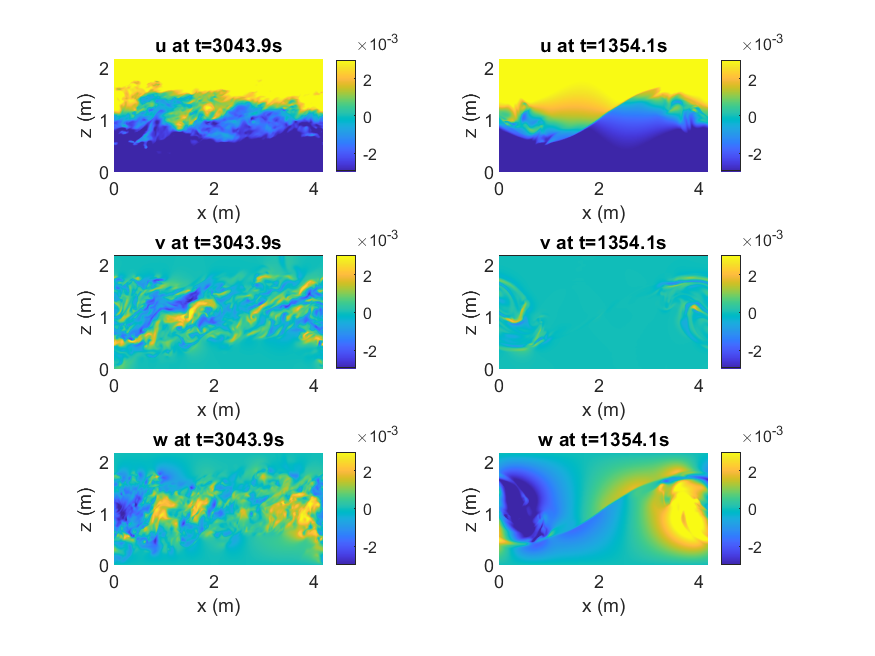
\includegraphics[width=\textwidth]{1-plots/Vel_plot_3043_1354.png}
				\caption{Instantaneous velocity at $t=\SI{3043.9}{\second}$ and at $t=\SI{1354.1}{\second}$.}
				\label{fig:Vel}
			\end{figure}
		
			\begin{figure}[htbp]
				\centering
				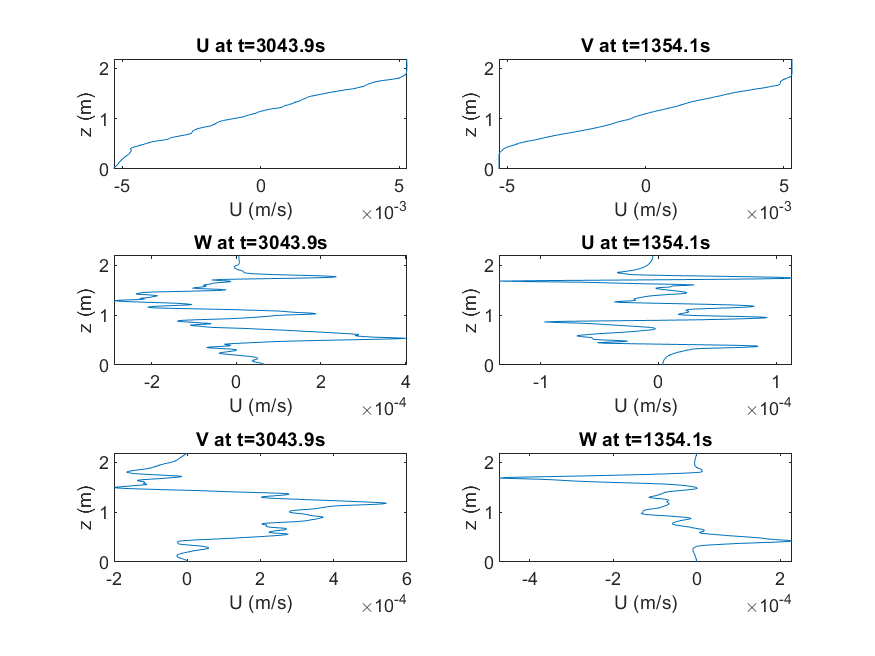
\includegraphics[width=\textwidth]{1-plots/Vel_avg_plot_3043_1354.png}
				\caption{Mean velocity at $t=\SI{3043.9}{\second}$ and at $t=\SI{1354.1}{\second}$.}
				\label{fig:Vel avg}
			\end{figure}
		
			\begin{figure}[htbp]
				\centering
				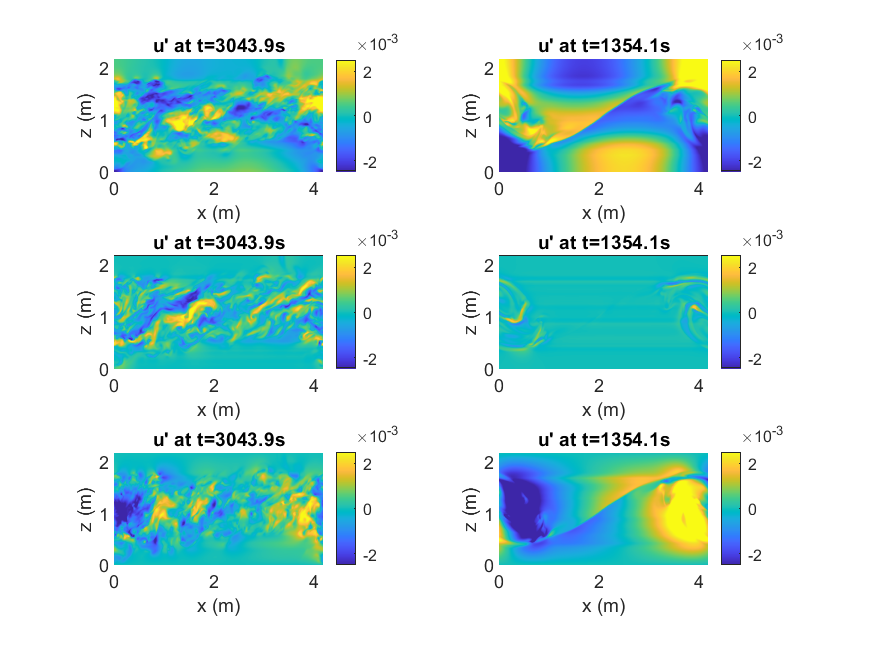
\includegraphics[width=\textwidth]{1-plots/Vel_primes_plot_3043_1354.png}
				\caption{Fluctuating velocity at $t=\SI{3043.9}{\second}$ and at $t=\SI{1354.1}{\second}$.}
				\label{fig:Vel prime}
			\end{figure}
			
			
			\clearpage
			\item Now that you have decomposed the velocity, compute the individual components of the turbulent kinetic energy and the Reynolds stresses. Discuss any significant features of the patterns or magnitudes.\par
			
			To calculate the TKE and the Reynolds stresses, I multiplied the fluctuating velocities together at each point in the time step. For the TKE, shown in \Cref{fig:tke}, I plotted the individual components, as well as the total TKE as functions of $x$ and $z$. The TKE in the $y$-direction has the smallest magnitude, which is what we would expect from this flow. The TKE in the $x$ direction looks a little more spread out than in the $z$ direction, but with similar magnitudes. \Cref{fig:reynolds 3043} shows the components of the Reynolds stress, without being multiplied by density. Similarly to the TKE, the Reynolds stresses with $y$ components included are smaller in magnitude than the other components.
			
			\begin{figure}[htpb]
				\centering
				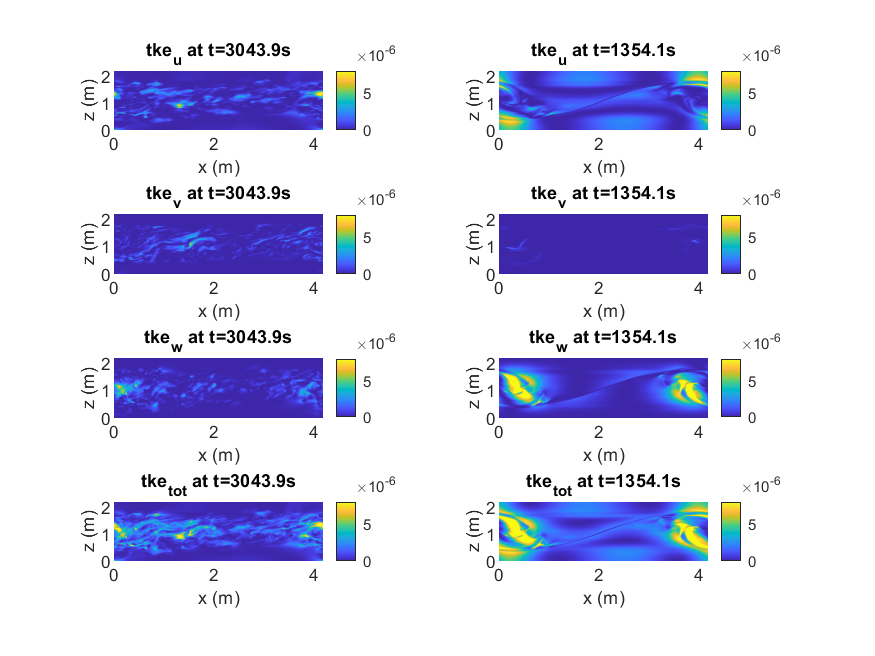
\includegraphics[width=\textwidth]{1-plots/tke_plot_3043_1354.png}
				\caption{TKE at $t=\SI{3043.9}{\second}$ and at $t=\SI{1354.1}{\second}$.}
				\label{fig:tke}
			\end{figure}
		
			\begin{figure}[htbp]
				\centering
				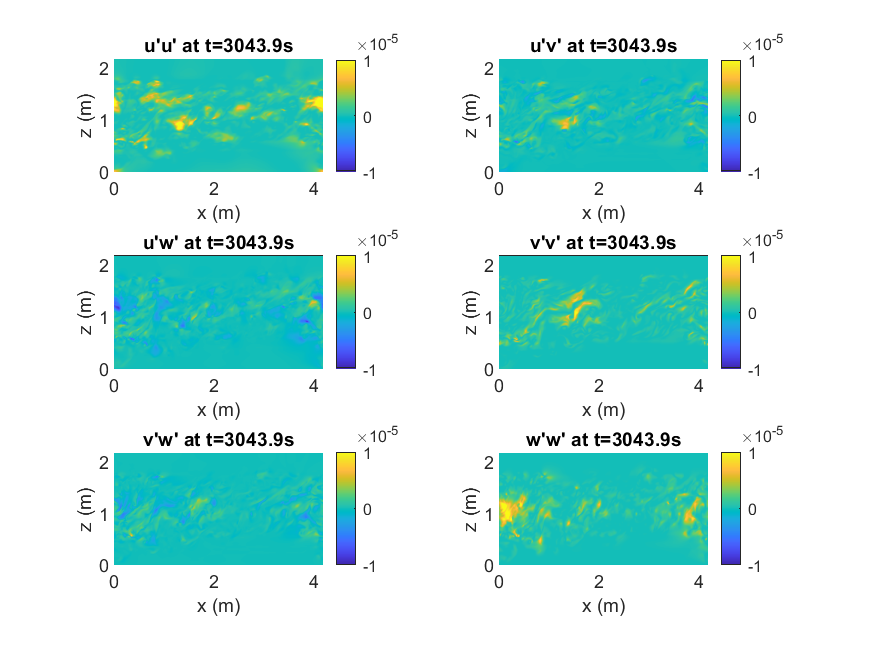
\includegraphics[width=\textwidth]{1-plots/ReynoldsStress_plot_3043.png}
				\caption{Reynolds stresses at $t=\SI{3043.9}{\second}$.}
				\label{fig:reynolds 3043}
			\end{figure}
			
			\clearpage
			\item Perform the same set of calculations for an earlier time in the flow (when the turbulence is perhaps less homogeneous). Discuss any differences in the character of the flow and/or the components of the tke and Reynolds stresses.\par
			
			I selected the third time step ($t=\SI{1354.1}{\second}$) to compare to the first selected time step because it is in a sweet spot where the flow is moving, but is not very turbulent. You can see over all of the plots above, and \Cref{fig:reynolds 1354} below, that the flow at the earlier time step is a lot less turbulent. It has structure and you can still see the two layers of flow and the boundary between them. Something else that is worth mentioning is the $y$-direction components are very small at the early time step, but increase for the later time step. We expect this due to the three-dimensional nature of turbulence.
			
			\begin{figure}[htbp]
				\centering
				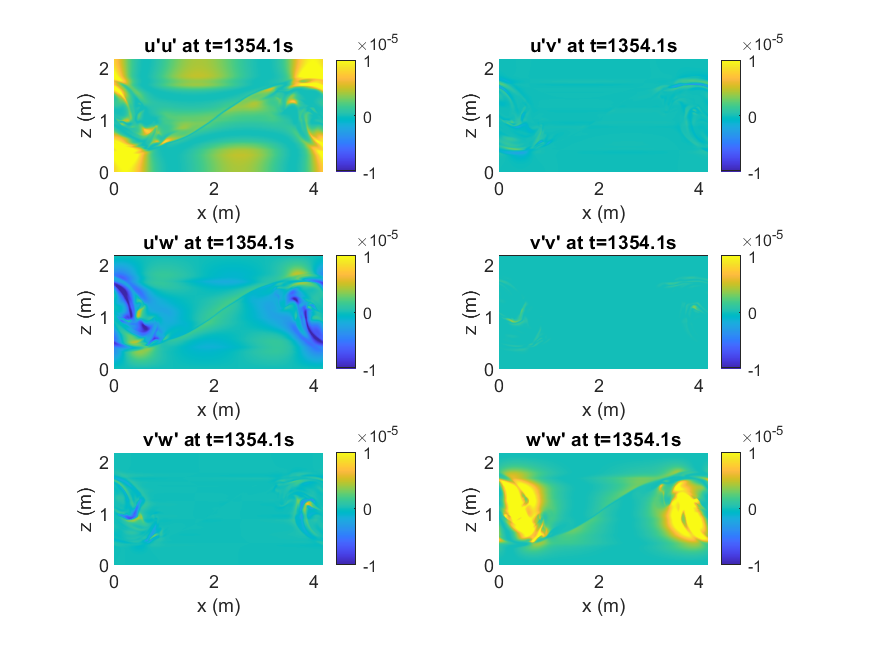
\includegraphics[width=\textwidth]{1-plots/ReynoldsStress_plot_1354.png}
				\caption{Reynolds stresses at $t=\SI{1354.1}{\second}$.}
				\label{fig:reynolds 1354}
			\end{figure}
			
			
			
		\end{enumerate}
	
		\clearpage
		% Part 2
		\item \textbf{Part 2:} For now neglect the buoyancy contributions and
		\begin{enumerate}
			\item compute the shear production and dissipation throughout the domain at some point in time. Determine a horizontal and volume average of each. Does production balance dissipation?\par
			
			This is the part that I am most unsure about currently. I am not sure that I am calculating $S_{ij}$ and $s_{ij}$ correctly. Beginning with the definitions of shear production and dissipation from the TKE equation, we have:
			\begin{equation}
				P = - \overline{u_i u_j} S_{ij}\:,
				\label{eq:production}
			\end{equation}
			and
			\begin{equation}
				\epsilon = 2\nu \overline{s_{ij} s_{ij}}\:.
				\label{eq:dissipation}
			\end{equation}
			Because the other terms are very small, $S_{ij}$ is only dependent on the $z$ derivative of the mean velocity in the $x$-direction.
			\begin{equation}
				S_{ij} =  \frac{\partial U}{\partial z}
			\end{equation}
			To calculate the production term, I used the Reynolds stress term, $u^{\prime}w^{\prime}$, and the $S_{ij}$ definition above.
		
			The fluctuating term needs all of the components because at the small scale, all of the components have significant contribution. It should be noted that I did not include any $y$ derivatives for any of my calculations because I only included one $y$ plane. This assumption may have effects on the fluctuating values, but I did not include it in my calculations when I first began and did not have the time to add it back in. 
			\begin{equation}
				s_{ij} = \frac{1}{2} \left( \frac{\partial u^{\prime}_i}{\partial x_j} + \frac{\partial u^{\prime}_j}{\partial x_i} \right)
			\end{equation}
			To calculate the dissipation, I squared the $s_{ij}$ matrix element-wise, then added the terms together, then multiplied that result by the viscosity. I am not sure that I did this correctly, especially because I probably made errors while coding it in MATLAB. \Cref{fig:prod diss 3043} shows the production and dissipation as functions of $x$ and $z$. The general shape and location of the dissipation matches the production pretty well, but the magnitude is smaller. Part of this difference may be due to me leaving out the $y$ terms, as well as me most likely messing up the calculation. To average the production and dissipation, I averaged over $x$ for each $z$ for the horizontal average (the same type of average as I performed for the velocity); for the volume average, I averaged the horizontal average values together to get one number. \Cref{fig:prod diss horiz} shows the horizontal average and \Cref{fig:prod diss jb time} shows the volume averages for all time steps. For the horizontal average, the production and dissipation do not look like they match each other, however, the dissipation does follow the same trend and the production if you remember that the dissipation is always positive due to squaring the components. So the magnitudes do not compare, but the shape is similar between the production and the dissipation at this time step.
			
			
			\begin{figure}[htbp]
				\centering
				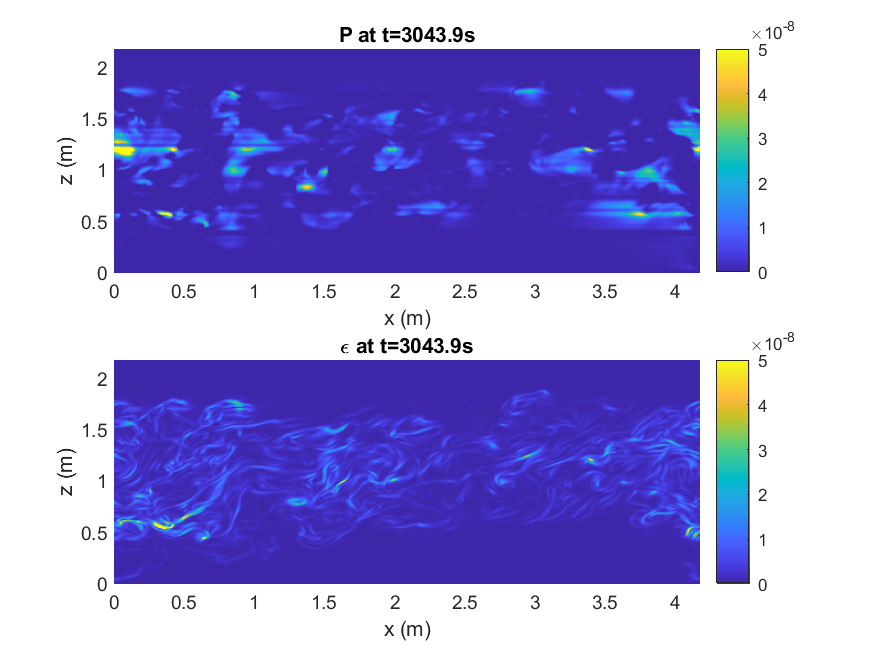
\includegraphics[width=\textwidth]{1-plots/prod_diss_plot_3043.png}
				\caption{Production and dissipation at $t=\SI{3043.9}{\second}$.}
				\label{fig:prod diss 3043}
			\end{figure}
			
			
			\begin{figure}
				\centering
				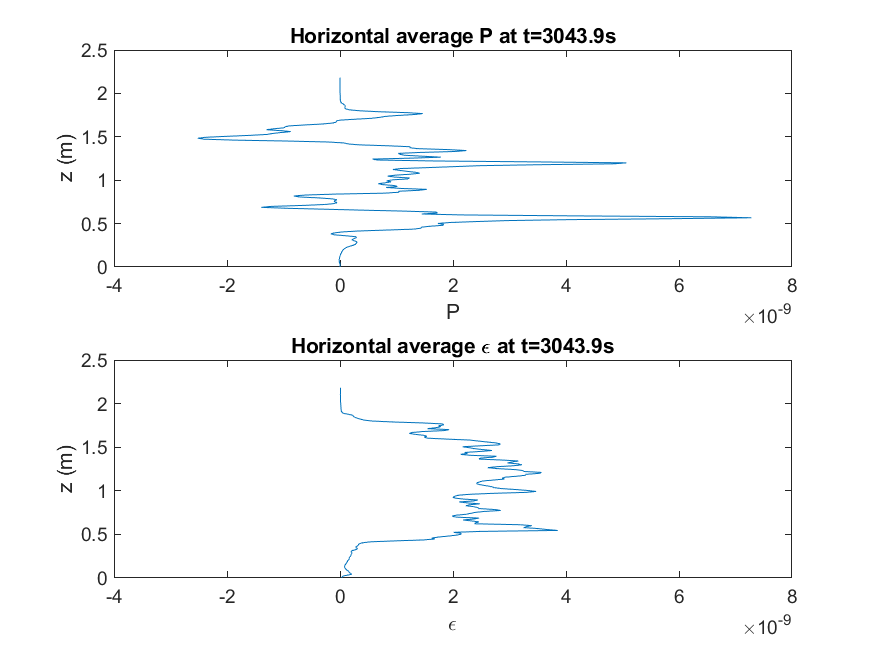
\includegraphics[width=\textwidth]{1-plots/Horizontal_prod_diss_plot_3043.png}
				\caption{Horizontal averaged shear production and dissipation at $t=\SI{3043.9}{\second}$.}
				\label{fig:prod diss horiz}
			\end{figure}
			
			
			
			\clearpage
			\item Once you are satisfied that you can compute production and dissipation (i.e., (a) above), compute the average of each for every timestep and plot a time series. Does production equal dissipation on average? Write a paragraph describing the production and dissipation evolution.\par
			
			\Cref{fig:prod diss jb time} shows the evolution over time of the volume averages of the shear production, dissipation, and the buoyancy production. Just looking at the beginning of the time evolution, we can see that the dissipation does not equal the production. However, after the production trends to zero at around \SI{1800}{\second} or so. After this point, the dissipation is pretty close to being equal to the production. As we would expect with no source adding to the turbulence, both the production and dissipation fall off as time goes on. At the beginning, the dissipation is small due to most of the energy being in the large scales, not having cascaded down to the small scales yet.
			
			
			\begin{figure}[htbp]
				\centering
				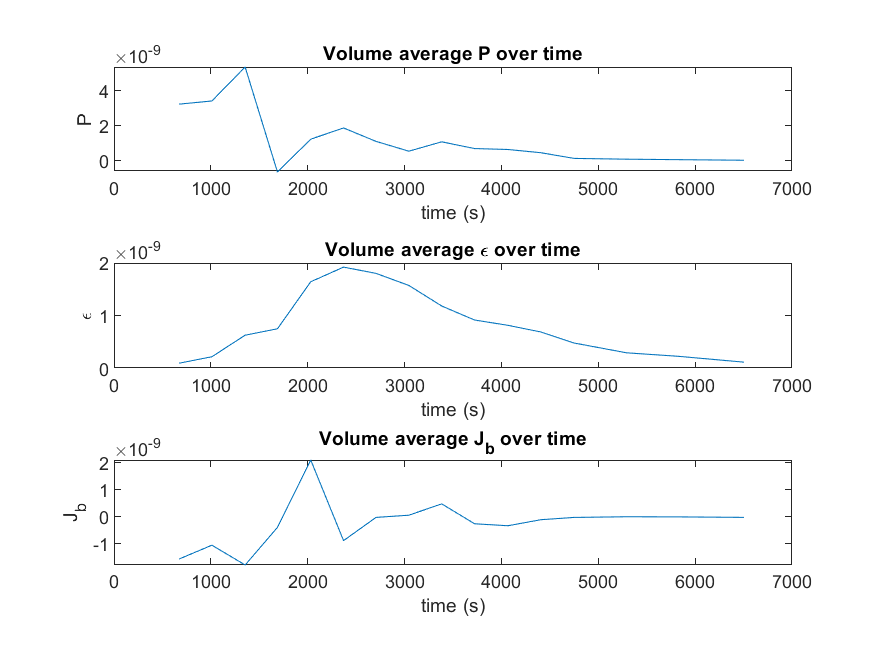
\includegraphics[width=\textwidth]{1-plots/Time_prod_diss_Jb_plot.png}
				\caption{Volume averaged shear production, dissipation, and buoyancy flux over time.}
				\label{fig:prod diss jb time}
			\end{figure}
		\end{enumerate}
	
	
		\clearpage
		% Part 3
		\item \textbf{Part 3:} Now consider the buoyancy production term.
		\begin{enumerate}
			\item Compute time-integrals of the spatially-integrated buoyancy production $J_b$ and compare this to shear production and dissipation. Does this help to account for any mismatches above? If there are mismatches and you can't close the energy budget, explain what might be the problem.\par
			
			To calculate the buoyancy production, I used the following definition.
			\begin{equation}
				J_b = -\frac{g}{\rho_0} \overline{w^{\prime}\rho^{\prime}}
			\end{equation}
			Both of the density values were provided by the data set, so no averaging or calculation was required. \Cref{fig:prod diss jb time} shows the evolution of the buoyancy production along with the shear production and the dissipation. It looks like the buoyancy does make up the difference between the dissipation and the production, especially at the beginning of the time evolution. Later on in time, it is difficult to tell just from the plot what contribution the buoyancy has, since it is close to zero. I did not explicitly calculate energy budget, so I do not know for sure how close it is. If it is not closed, the error from not including the $y$ derivative terms might the greatest factor. Also, I could have calculated something wrong.
			
			
			\item  Now try to compare these to the integrated TKE production and the total change in potential energy due to mixing within the simulation domain. Can you close an energy budget, and if not, what might be the problem? What is the mixing efficiency? Which measure of the total mixing is most robust?\par
			
			To calculate the mixing efficiency, I used the following formula:
			\begin{equation}
				\Gamma = \frac{J_b}{\epsilon}\:.
			\end{equation}
			\Cref{tab:mixing} shows the volume averaged mixing efficiency for each time step. It does not make sense to be negative, so I maybe should have taken the absolute value, but the magnitudes look mostly reasonable. Some of them are very high, but that might be due to the averaging not properly capturing the mixing.
			
			
			
			\begin{table}[htbp]
	\centering
	\caption{Volume average mixing efficiency.}
	\begin{tabular}{cc}
	\toprule
	 Time (s) & $\Gamma$\\ 
	\midrule
	 6.718e+02 & -14.308 \\ 
	 1.010e+03 & -4.550 \\ 
	 1.354e+03 & -2.798 \\ 
	 1.688e+03 & -0.513 \\ 
	 2.031e+03 & 1.282 \\ 
	 2.370e+03 & -0.458 \\ 
	 2.705e+03 & -0.011 \\ 
	 3.044e+03 & 0.039 \\ 
	 3.383e+03 & 0.406 \\ 
	 3.723e+03 & -0.277 \\ 
	 4.067e+03 & -0.399 \\ 
	 4.406e+03 & -0.151 \\ 
	 4.750e+03 & -0.042 \\ 
	 5.291e+03 & 0.015 \\ 
	 5.827e+03 & -0.003 \\ 
	 6.505e+03 & -0.146 \\ 
	\bottomrule
	\end{tabular}
	\label{tab:mixing}
\end{table}
		
		\end{enumerate}
		
	\end{enumerate}
		
	
	
	
	
	
	
	
	
	
\end{document}